\chapter{Fatores Relevantes da Implementação de algoritmos baseados em KDE}\label{cap:algoritmo}

Neste capítulo, serão descritos alguns detalhes de construção do algoritmo de identificação de partículas desenvolvido no âmbito dessa tese e, além disso, serão ilustrados casos onde é possível otimizar a estimação via KDE. A estimação da densidade conjunta das variáveis discriminantes é central para o método de Verossimilhança e, devido a isto, este trabalho se concentrou neste tópico, a fim de indicar possíveis caminhos na definição de uma metodologia a ser adotada na implementação do KDE.

\section{Algoritmo}

O algoritmo de identificação de partículas baseado no método de verosimilhança pode ser resumido pelo diagrama de blocos da Figura \ref{fig:08}. Inicialmente são escolhidas as informações discriminantes, as variáveis do detector que serão utilizadas, como já mencionado na Seção \ref{sec:menu}, depois disso, é feita a estimação de densidade unidimensional e bidimensional (quando for o caso), com as PDF marginais faz-se o cálculo da PDF conjunta, aplica-se o discriminante e por fim retira-se a informação de classificação pelos índices \ac{SP}, dado pela Equação \ref{eq:07}, e \ac{AUC} \cite{bradley1997use}. Todo o processo é feito para cada região da Tabela \ref{tab:5T01} individualmente.

\begin{figure}[!ht]
	\begin{center}
		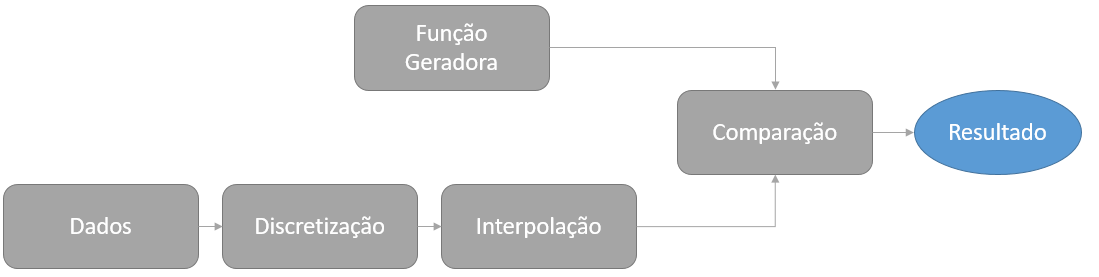
\includegraphics[width=0.9\linewidth]{./figuras/algoritmo1.png}
		\caption{Diagrama de blocos da utilização do método de Verossimilhança com as variáveis do \textit{Ringer}.}\label{fig:08}
	\end{center}
\end{figure}

\begin{equation}\label{eq:07}
    SP = \sqrt {\left( {\sqrt {VP \cdot FP} } \right) \cdot \left( {\frac{{VP + FP}}{2}} \right)}
\end{equation}
onde $VP$ e $FP$ são os valores de Verdadeiros Positivos e Falso Positivo, respectivamente, retirados da curva \ac{ROC}, que demonstra o desempenho de um sistema classificador binário.

\subsection{Validação Cruzada}

Todas as análises apresentadas aqui foram realizadas usando \ac{CV}. Segundo \cite{kohavi1995study}, a validação cruzada visa garantir a generalização do modelo proposto, evitando problemas como super-aprendizado ou super-ajuste. A implementação da \ac{CV} foi baseada em \textit{K-fold}, esse método consiste em separar o conjunto de dados em $k$ blocos e utilizar $k-1$ blocos para o conjunto de treinamento do algoritmo e o bloco restante para o conjunto de validação. Essa abordagem é repetida $k$ vezes alternando os blocos, como mostrado na Figura \ref{fig:09}. No caso desse trabalho foi escolhido o $k$ igual a 10, de acordo com o aconselhado por \cite{kohavi1995study}.

\begin{figure}[!ht]
	\begin{center}
		\includegraphics[width=0.45\linewidth]{./figuras/Kfold.png}
		\caption{Esquemático da validação cruzada baseada em \textit{k-fold}.}\label{fig:09}
	\end{center}
\end{figure}

\section{Alguns pontos para otimização do algoritmo de estimação de densidades}

Como citado anteriormente na Seção \ref{cap:rev} existem alguns tópicos de interesse na literatura com relação a otimização de algoritmos de estimação de densidades, alguns desses fora do escopo de estimação em si, mas não menos cruciais para o melhor desempenho dessa ferramenta. No caso dessa tese, visando otimização do processos de estimação e identificação de partículas, foram abordados os temas de Custo computacional, \textit{Outliers} e Discretização, que serão melhores discutidos nas seções subsequentes.

\subsection{Custo Computacional}

Os algoritmo de \textit{Kernel} são muito utilizados na literatura no contexto de análise de dados ou modelagem de dados, entretanto é sabido que esse método é computacionalmente mais lento em comparação com outros. Por isso muitos pesquisadores fazem uso de algoritmos que efetuam aproximações matemáticas no intuito de ganhar em custo computacional, chamados de \textit{FastKDE}, ou seja, existe um \textit{trade-off} entre estabilidade numérica e economia computacional. Entretanto, como o objetivo aqui é fazer uso da maior precisão numérica possível, foi desenvolvido nessa tese um algoritmo de KDE que efetua os cálculos de forma matricial, com isso há uma diminuição relevante de \textit{loopings} no algoritmo o que consequentemente colabora para a economia computacional, além disso, há ainda a possibilidade de dividir as matrizes criadas, quando o número de eventos for grande, efetuando o processamento em paralelo. Essas características fazem com que o KDE seja rápido e eficiente. 

Métodos de KDE comparados neste trabalho:

\begin{itemize}
\item KDE Naive (Banda Fixa) \cite{scott2015multivariate};
\item KDE Naive (Banda Variável) \cite{scott2015multivariate};
\item FastKDE (Banda Fixa);
\item FastKDE (Banda Variável);
\item KDE via Difussion (Banda Fixa) \cite{botev2010kernel};
\end{itemize}



Na Figura \ref{fig:compKDE} é apresentada uma comparação do método aqui desenvolvido com alguns métodos da literatura, em relação ao tempo de processamento e a Figura \ref{fig:erroKDE} mostra o erro de estimação de cada método. O primeiro gráfico varia em relação ao número de eventos e número de pontos de estimação, já o segundo varia somente em relação ao número de eventos, mantendo o número de pontos de estimação igual a 64, a distribuição estimada é a Gaussiana $N(0,1)$.

\begin{figure}[!ht]
	\centering
	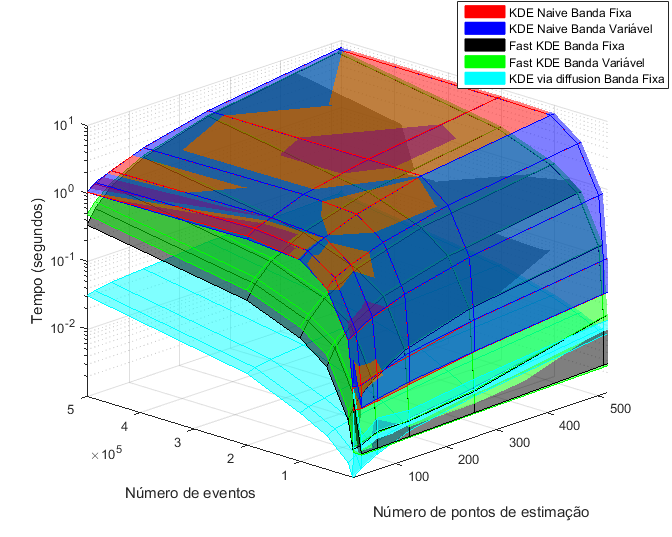
\includegraphics[width=12cm]{./textuais/desenvolvimento/figuras/compKDE.png}\\
	\caption{Comparação entre diferentes métodos de FastKDE em relação ao tempo de processamento, para uma distribuição Gaussiana.}
	\label{fig:compKDE}
\end{figure}

Pode-se notar que o \textit{FastKDE} implementado nesse trabalho apresenta o menor tempo de processamento em relação aos métodos que fazem uso de largura de banda variável e mesmo assim apresenta erro de estimação baixo. Para o caso ilustrado as estimações com largura de banda fixa atingem erros menores ao serem comparadas com os métodos de largura de banda variável, uma vez que esses são ótimos para uma distribuição Gaussiana \cite{scott2015multivariate}.

\begin{figure}[!ht]
	\centering
	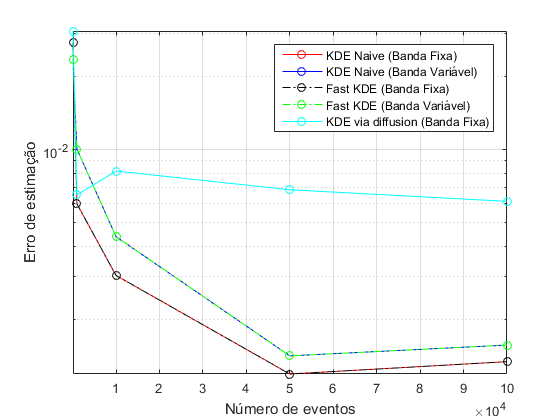
\includegraphics[width=12cm]{./textuais/desenvolvimento/figuras/erroKDE.png}\\
	\caption{Comparação entre diferentes métodos de KDE em relação ao erro de estimação, para uma distribuição Gaussiana.}
	\label{fig:erroKDE}
\end{figure}

Já quando o objetivo é estimar uma distribuição \textit{Lognormal} $Logn(0,0.8)$ nota-se que os estimadores que utilizam largura de banda variável atingem valores de erros menores que os outros, como mostrado na Figura \ref{fig:erroKDElog}. E o tempo de processamento dos métodos para a distribuição \textit{lognormal} pode ser visto na Figura \ref{fig:compKDElog}.

\begin{figure}[!ht]
	\centering
	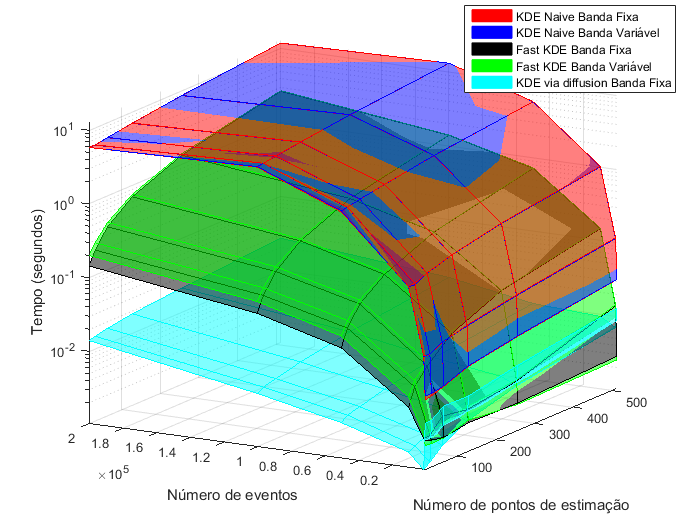
\includegraphics[width=12cm]{./textuais/desenvolvimento/figuras/compKDElog.png}\\
	\caption{Comparação entre diferentes métodos de FastKDE em relação ao tempo de processamento, para uma distribuição \textit{Lognormal}.}
	\label{fig:compKDElog}
\end{figure}

\begin{figure}[!ht]
	\centering
	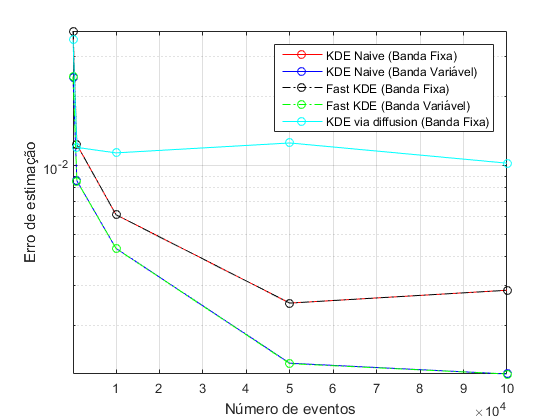
\includegraphics[width=12cm]{./textuais/desenvolvimento/figuras/erroKDElog.png}\\
	\caption{Comparação entre diferentes métodos de KDE em relação ao erro de estimação, para uma distribuição \textit{Lognormal}.}
	\label{fig:erroKDElog}
\end{figure}

\clearpage

\subsection{Descontinuidades e \textit{Outliers}}

O pré-processamento dos dados é utilizado para a remoção de descontinuidades e \textit{outliers} presentes nos histogramas das variáveis discriminantes. Sendo o primeiro um efeito que ocorre, principalmente, por indeterminações matemáticas no processo de cálculo das probabilidades, como por exemplo, divisão por zero, já os \textit{outliers} são eventos que ocorrem na região de baixa probabilidade, distantes da região central da PDF. Exemplos desses efeitos são mostrados no caso representativo da Figura \ref{fig:5T06}.

  \begin{figure}[h]
	\centering
	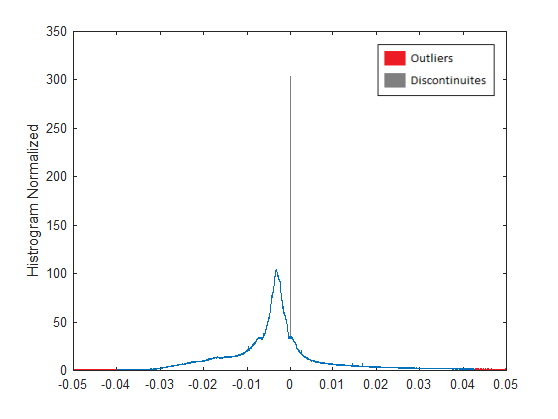
\includegraphics[width=10cm]{./textuais/algoritmo/figuras/explicacaooutilers.png}\\
	\caption{Gráfico da distribuição de uma variável, exemplificando os Valores Extremos (\emph{Outliers}) e Descontinuidades (\emph{Discontinuites}).}
	\label{fig:5T06}
\end{figure}


\subsection{Discretização}

Atualmente os algoritmos de estimação de densidade via KDE utilizam a discretização com espaçamento uniforme, ou seja, depois de feita a estimação faz-se necessário escolher alguns pontos que serão armazenados para representar aquela distribuição, nesse momento monta-se uma grade de pontos distribuídos uniformemente no eixo das abscissas. Entretanto, fazer o uso desse espaçamento para variáveis que não são gaussianas pode contribuir para uma estimação não-otimizada das distribuições. Em \cite{costa2017study} é feito um estudo sobre a utilização de 4 métodos de escolha da discretização da grade, sendo um deles baseado na \ac{CDF}, que podem tornar a estimação de densidades menos suscetível a \textit{outliers} e distribuições com longas caudas. Na Figura \ref{fig:linspace}, é ilustrado o funcionamento do método linear (padrão na literatura) e do método baseado na \ac{CDF}.

\begin{figure}[H]
		\centering
		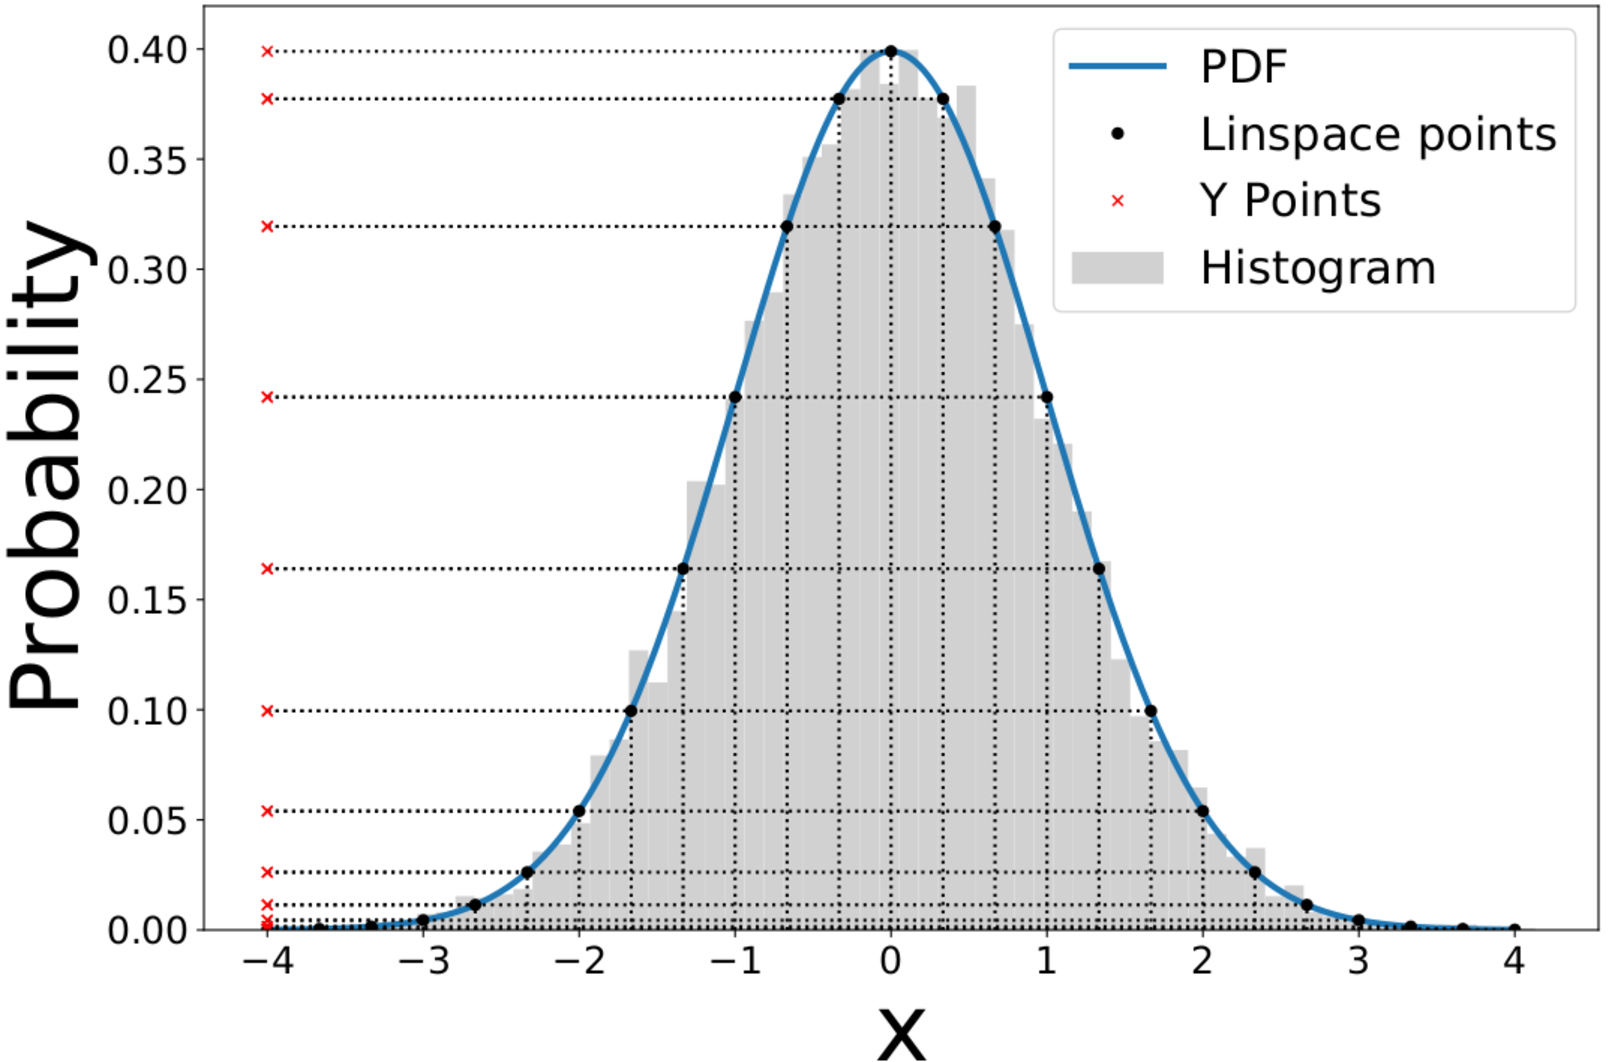
\includegraphics[width=7cm]{./textuais/algoritmo/figuras/2.pdf}
        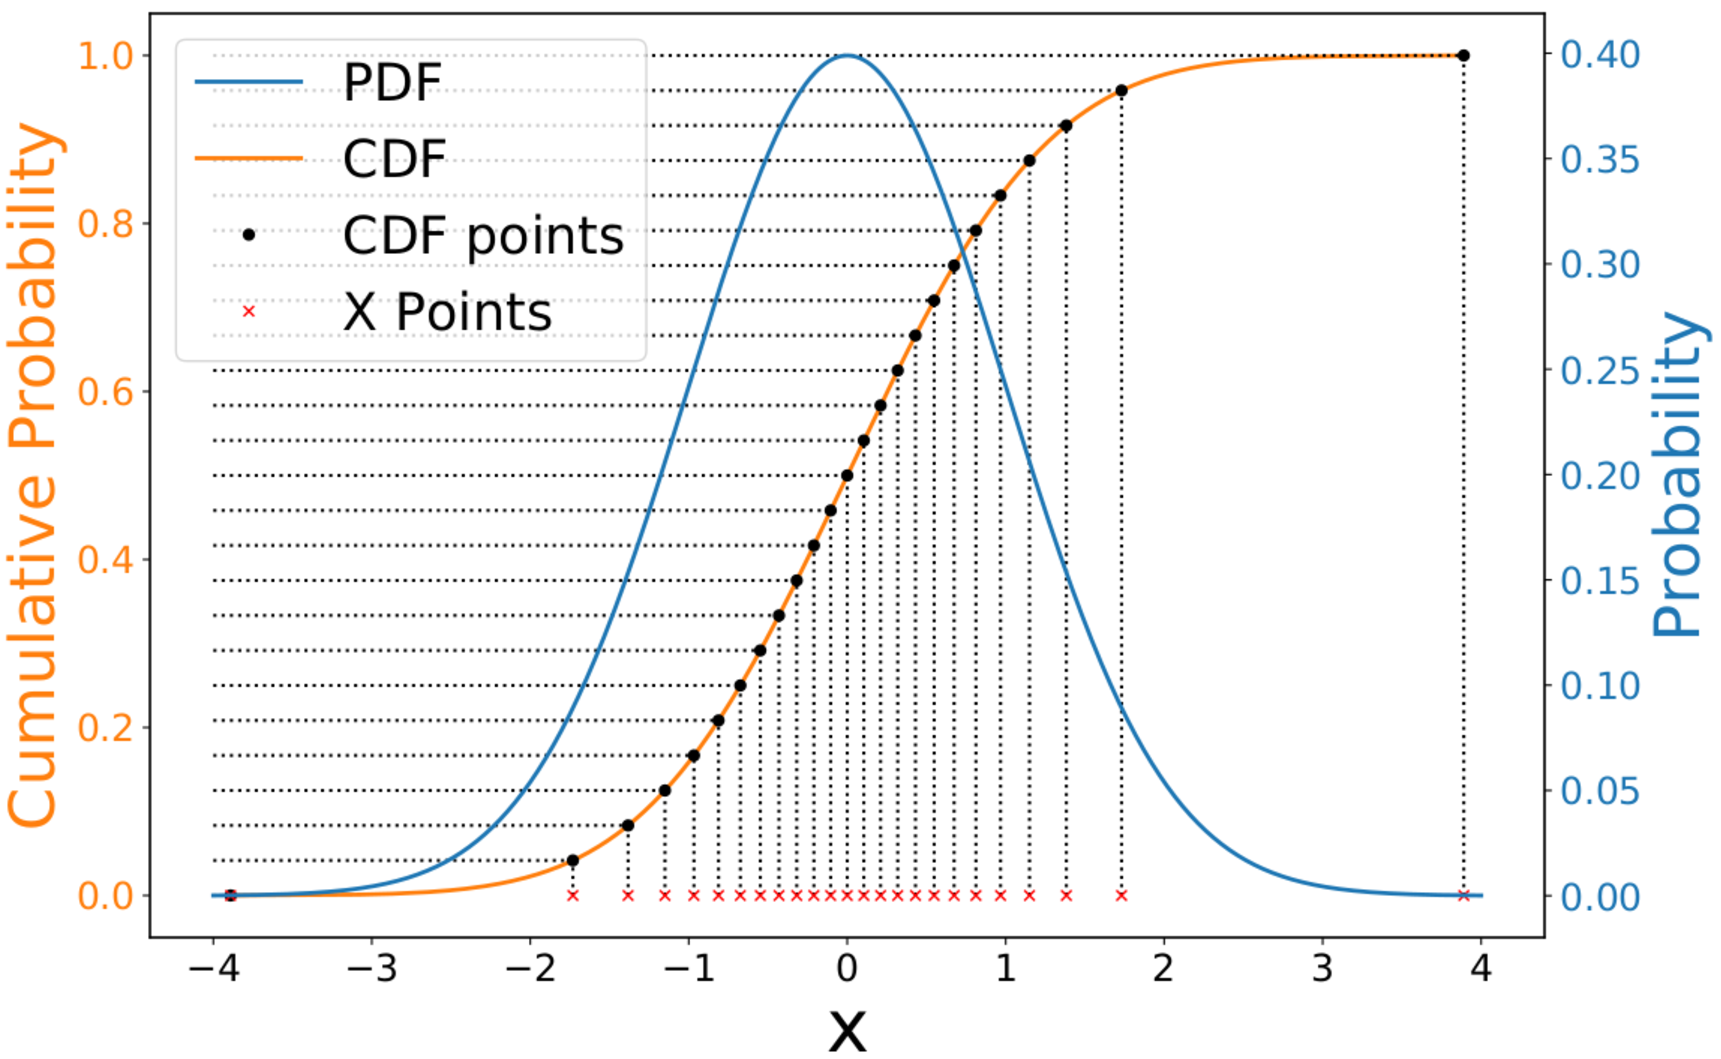
\includegraphics[width=7.5cm]{./textuais/algoritmo/figuras/1.pdf}
		\caption{Caso representativo do método de discretização baseado no espaçamento linear (Esquerda) e baseado na \ac{CDF} (Direita) aplicado a uma distribuição Gaussiana.}
		\label{fig:linspace}
\end{figure}

Essa ferramenta está sendo avaliada em um ambiente controlado, utilizando de distribuições parametrizadas, para ter conhecimento de todas as suas características e, então, será testada no ambiente de física de altas energias.

\section{Estimação de densidades das regiões de interesse} \label{sec:difest}

A implementação do algoritmo baseia-se nas formulações matemáticas descritas na Seção~\ref{sec:kdeuni}. Nessa abordagem, é considerado um KDE com banda variável otimizado através do parâmetro $\lambda$, de acordo com a otimização apresentada na Seção~\ref{sec:bandavariavel}, restando utilizar o histograma, com a binagem escolhida baseada no algoritmo proposto por \cite{shimazaki2007method}, para calcular o valor de $f\left( x \right)$ de cada evento, como mostrado na equação~\ref{eq:54}.

Computacionalmente, no processo de estimação das densidades, deve-se escolher o número de pontos a ser usado para a sua representação discreta. Adicionando esse número aos parâmetros mencionados no parágrafo anterior, as PDF podem ser construídas através do método de KDE. O algoritmo implementado foi programado para gerar 2000 pontos para cada variável, de maneira a garantir uma boa representação de suas respectivas distribuições. Os valores das variáveis gerados pelos eventos de colisão são, então, interpolados linearmente a partir dos pontos da PDF discreta.

As Figuras~\ref{fig:9T20} até~\ref{fig:9T23} mostram alguns casos representativos das distribuição a serem estimadas pelo algoritmo de KDE na Região 4 (Esquerda) e Região 15 (Direita), para o conjunto de sinal (denominado \emph{electron}, por ser formado por elétrons isolados) e para o conjunto de ruído de fundo (denominado \emph{Jet}, pela predominância de jatos). A escolha da melhor binagem para visualização do \ac{ASH} foi feita utilizando o método de Freedman-Diaconis \cite{freedman1981histogram}.

\begin{figure}[H]
	\centering
	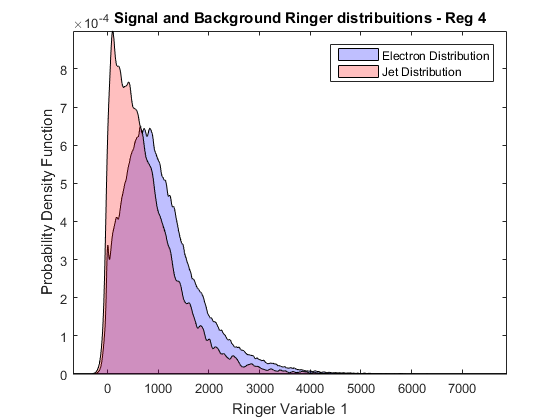
\includegraphics[width=7cm]{./textuais/algoritmo/figuras/DISTKERNELET3ETA0VAR1KF1.png}
    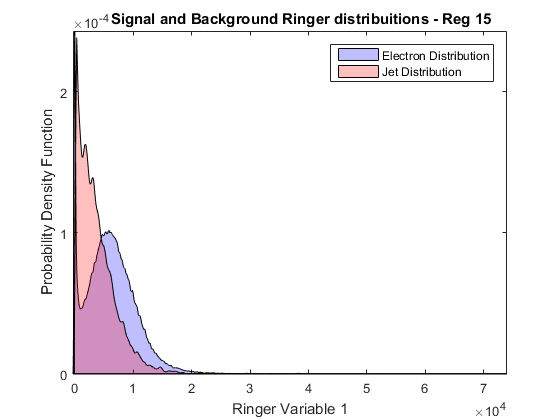
\includegraphics[width=7cm]{./textuais/algoritmo/figuras/DISTKERNELET4ETA2VAR1KF1.png}\\
	\caption{Gráficos das distribuições de elétron e jato do anel 1. (Esquerda) Região 4 e (Direita) Região 15.}
	\label{fig:9T20}
\end{figure}

\begin{figure}[H]
	\centering
	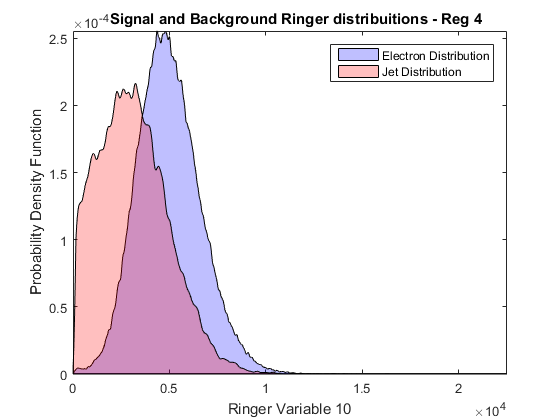
\includegraphics[width=7cm]{./textuais/algoritmo/figuras/DISTKERNELET3ETA0VAR10KF1.png}
    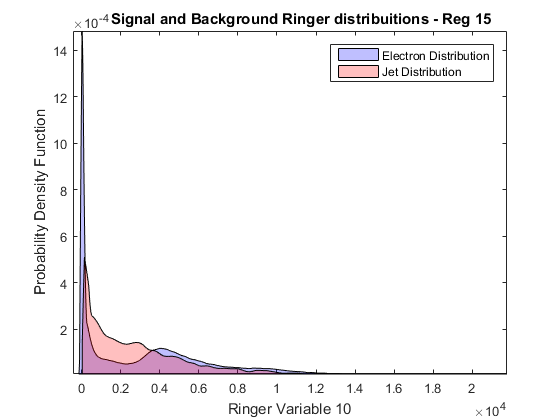
\includegraphics[width=7cm]{./textuais/algoritmo/figuras/DISTKERNELET4ETA2VAR10KF1.png}\\
	\caption{Gráficos das distribuições de elétron e jato do anel 10. (Esquerda) Região 4 e (Direita) Região 15.}
	\label{fig:9T21}
\end{figure}

\begin{figure}[H]
	\centering
	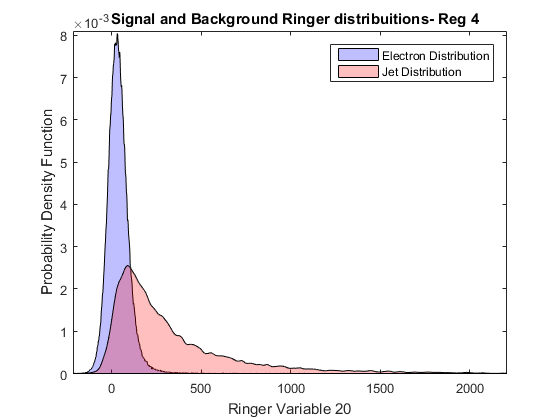
\includegraphics[width=7cm]{./textuais/algoritmo/figuras/DISTKERNELET3ETA0VAR20KF1.png}
    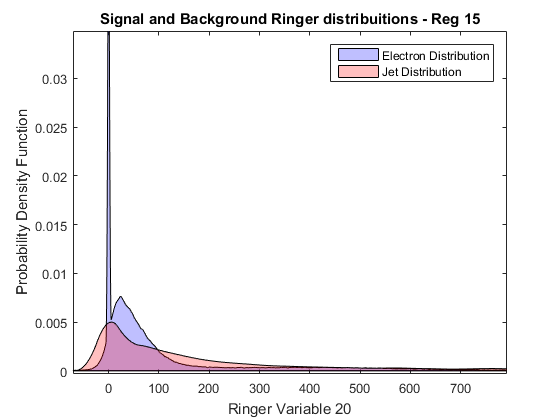
\includegraphics[width=7cm]{./textuais/algoritmo/figuras/DISTKERNELET4ETA2VAR20KF1.png}\\
	\caption{Gráficos das distribuições de elétron e jato do anel 20. (Esquerda) Região 4 e (Direita) Região 15.}
	\label{fig:9T22}
\end{figure}

\begin{figure}[H]
	\centering
	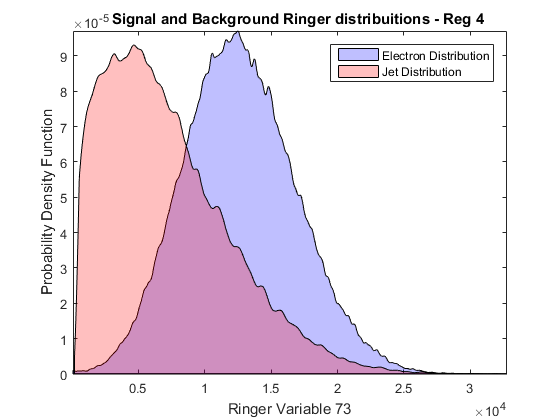
\includegraphics[width=7cm]{./textuais/algoritmo/figuras/DISTKERNELET3ETA0VAR73KF1.png}
    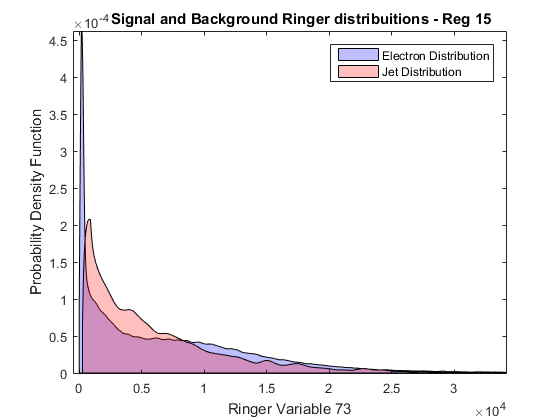
\includegraphics[width=7cm]{./textuais/algoritmo/figuras/DISTKERNELET4ETA2VAR73KF1.png}\\
	\caption{Gráficos das distribuições de elétron e jato do anel 73. (Esquerda) Região 4 e (Direita) Região 15.}
	\label{fig:9T23}
\end{figure}

De acordo com as Figuras~\ref{fig:9T20} até~\ref{fig:9T23} temos que as distribuições das variáveis discriminantes provenientes da Região 4 tem transições mais suaves, não possuem mais de um cume, tem derivadas e caudas menores em comparação com as distribuições obtidas da Região 15. Esse detalhe faz com que a estimação das PDF da Região 15 seja mais complexa, demandando algoritmos mais robustos e com características particulares, além disso a Região 15 contém 6 vezes menos estatística do que a Região 4, de acordo com a Tabela \ref{tab:5T01}, isso significa que existe a exigência de uma performance ótima mesmo com pouca estatística. Tais dificuldades abrem caminho para a pesquisa na direção de otimização de algoritmos de estimação de densidades baseado em núcleo.

Além disso, as variáveis provenientes de sensores similares, calorímetros por exemplo, são mais propensas a apresentar correlação mútua, como é o caso das variáveis de \textit{Ringer}, como pode ser visto nas Figuras \ref{fig:9T24} e \ref{fig:9T25}, isso faz com que o uso de todas as 100 variáveis ao mesmo tempo ocasione um erro devido a simplificação adotada do método de verossimilhança, que faz a suposição de independência entre as variáveis.

\begin{figure}[H]
	\centering
	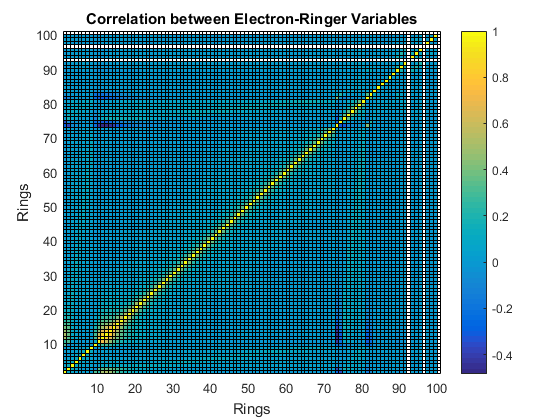
\includegraphics[width=12cm]{./textuais/algoritmo/figuras/plotCorrElectron.png}\\
	\caption{Gráficos da correlação entre as variáveis do \textit{Ringer} para elétron.}
	\label{fig:9T24}
\end{figure}

\begin{figure}[H]
	\centering
    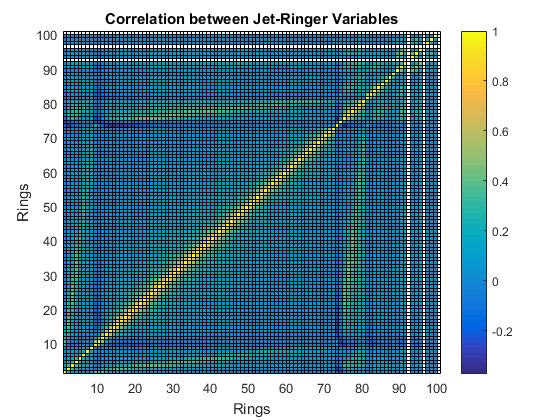
\includegraphics[width=12cm]{./textuais/algoritmo/figuras/plotCorrJet.png}\\
	\caption{Gráficos da correlação entre as variáveis do \textit{Ringer} para jato.}
	\label{fig:9T25}
\end{figure}

Portanto é necessário o uso de uma ferramenta para escolher quais anéis serão utilizados em cada região, no intuito de viabilizar a implementação desse algoritmo nas variáveis de \textit{Ringer}. A escolha pelo uso de uma técnica de busca utilizada para achar soluções aproximadas em problemas de otimização foi feita baseada na estrutura do problema em questão.

\section{Algoritmo Genético}

O \ac{GA} baseia-se em uma codificação do conjunto das possíveis soluções, apresenta os resultados como uma população de soluções, não necessita de nenhum conhecimento derivado do problema, mas somente de uma forma de avaliação do resultado (função a ser minimizada) e usa transições probabilísticas ao invés de regras determinísticas, tais características justificam a escolha dessa ferramenta para a escolha das variáveis discriminantes a serem utilizadas pelo algoritmo de identificação de elétrons.

O \ac{GA} utilizado embasa-se na implementação de \cite{haupt1998practical}, que é um Algoritmo Genético Binário e foi configurado alguns parâmetros para se adequar a realidade do problema em questão. Segue abaixo o \textit{setup} utilizado pelo \ac{GA}:

\begin{itemize}
\item Número máximo de iterações = $100$;
\item Tamanho da população = $60$ indivíduos;
\item Taxa de mutação = $2\%$;
\item Fração da população mantida entre cada iteração = $50\%$;
\item Número de bits no cromossomo = $100$;
\item População inicial = $1$;
\item Função custo = Minimização dos parâmetros SP ou AUC da classificação.
\end{itemize}

Esses parâmetros possibilitando que o \ac{GA} seja capaz de encontrar um dos melhores conjunto de anéis com a menor quantidade de anéis possível, visto que sua população inicial é igual a $1$, sua taxa de mutação é suficiente para escapar de mínimos locais, mas não grande ao ponto de tornar o algoritmo completamente aleatório. Esse método é utilizado no conjunto de treinamento para decidir quais anéis serão utilizados no conjunto de validação.

\section{Principais diferenças em relação ao método utilizado pela Colaboração ATLAS}

Como visto nas seções precedentes, a busca por uma otimização do algoritmo baseado no método de Verossimilhança a partir da estimação de densidades univariadas desenvolvida neste trabalho levaram a uma implementação ligeiramente diferente daquela em uso atualmente pela Colaboração. A Tabela~\ref{tab:5T02} resume as principais diferenças encontradas.

\begin{table}[H]
  \centering
  \caption{Tabela de diferenças entre a \ac{LH} da colaboração \cite{atlasdescription} e o algoritmo implementado nessa dissertação.}\label{tab:5T02}
\begin{tabular}{c|c|c}
  % after \\: \hline or \cline{col1-col2} \cline{col3-col4} ...
  & LH Colaboração Atlas & LH desse trabalho  \\ \hline \hline
  Método & Verossimilhança & Verossimilhança \\
  Variáveis & 13 & 106 \\
  Cortes Adicionais & Todos & Nenhum \\
  Interpolação & * & Linear \\
  Extrapolação & Vizinho mais próximo & Exponencial \\
  PDF & KDE & MKDE \\
  Regiões em $\eta$ e $E_t$ & 9x6 & 4x5 \\
  Pontos na PDF & 520** & 2000 \\
\end{tabular}

\begin{flushleft}
*A nota \cite{atlasdescription} não deixa clara a forma de interpolação utilizada.
**Para a variável TRT, utilizaram-se 62 pontos.
\end{flushleft}
\end{table}


Nesse capítulo foram apresentados os principais testes de definições relacionados ao algoritmo de classificação de partículas via método de verossimilhança com abordagem univariada utilizando as variáveis de \textit{Ringer}, bem como apontado as otimizações  que podem ser realizadas nele no intuito de se obter um melhor desempenho na classificação dos eventos. No Capítulo~\ref{cap:Resultados} serão apresentados os resultados obtidos com a aplicação desses métodos nos dados de validação.
